\subsection{Fundamentos de convección}
De la ecuación de enfriamiento de Newton~\ref{eq:enfriamiento-newton}
se puede deducir que \textit{el coeficiente de transferencia de calor por convección}
es \textit{a corriente de calor causada por convección es aproximadamente proporcional a la potencia de la diferencia de temperatura entre la superficie y el cuerpo
principal del fluido}. 

Por otra parte Todas las observaciones experimentales indican que un fluido en movimiento llega a detenerse por completo en la superficie y toma una velocidad
cero con respecto a esta última. Es decir, un fluido en contacto directo con un
sólido “se adhiere” a la superficie debido a los efectos viscosos y no se desliza. Esto se conoce como la condición de no deslizamiento.

La región del flujo adyacente a la superficie en
la cual los efectos viscosos son significativos
se llama \textit{capa límite}. La propiedad
del fluido responsable de la condición de no desplazamiento 
y del desarrollo de la capa límite y \textit{viscosidad}.

Otra consecuencia de la condición de no d
desplazamiento es el \textit{Arrastre superficial}, 
el cual es la fuerza que un fluido ejerce sobre una superficie,
en la dirección del flujo.

Una implicación de la condición de no desplazamiento es que la transferencia
de calor de la superficie del sólido hacia la capa de fluido adyacente a esa superficie
se da pro \textit{conducción} pura, ya 
que la capa de fluido está inmóvil, y se puede expresar como

\begin{equation}
    \dot{q} = -k_{fluido}\frac{\partial T}{\partial y}|_{y=0}
\end{equation}

donde $T$ representa la distribución de temperatura en el fluido
y ${(\partial T / \partial y)}_{y=0}$ es el \textit{gradiente de temperatura en la superficie.}
A continuación, este calor \textit{se aleja por convección} de
la superficie como resultado del movimiento del fluido.

\begin{figure}[ht]
    \begin{center}
        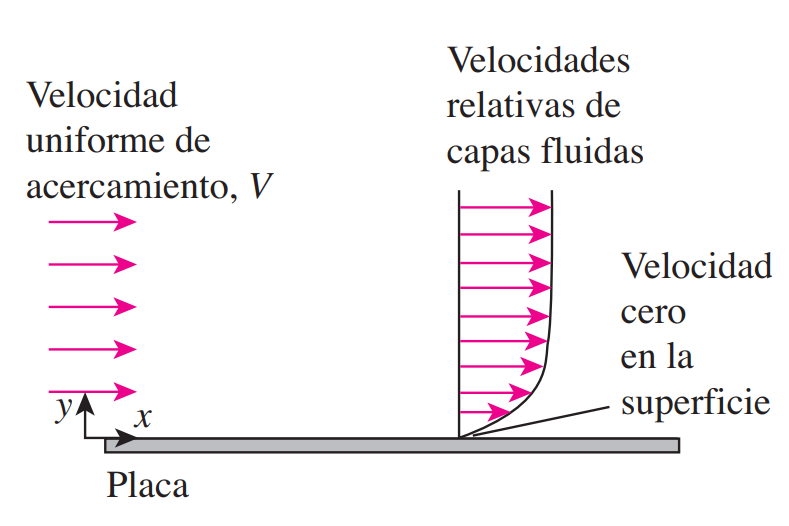
\includegraphics[width=0.5\textwidth]{img/f1.png}
    \end{center}
    \caption{Un fluido que fluye sobre una superficie estacionaria
    llega a detenerse por completo en la superficie a causa de la condición de no deslizamiento}
\end{figure}

\subsection{Número de Nusselt}
Con una conductividad térmica $k$ de un fluido
y $L_c$ la longitud característica, como se 
observa en la figura.

\begin{figure}[ht]
    \begin{center}
        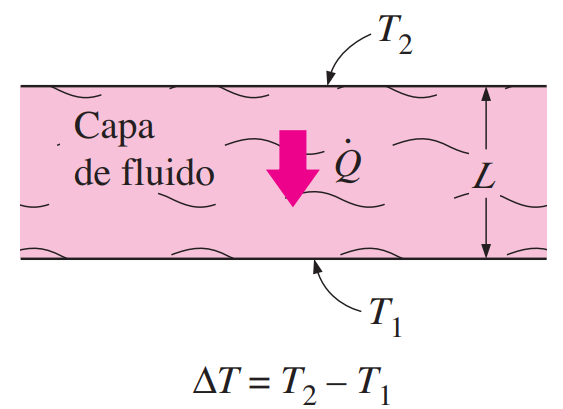
\includegraphics[width=0.3\textwidth]{img/f2.png}
    \end{center}
     
\end{figure}

Entonces el número de Nusslet se puede definir como

\begin{equation}
    \label{eq:nu:nusselt}
    N_u = \frac{h L_c}{k}
\end{equation}

Este número recibió el nombre en honor de Wilhelm Nusselt
se concibió como el \textit{coeficiente adimensional de
transferencia de calor por convección}




\subsection{Convección Externa Forzada}

La convección forzada es un mecanismo o tipo de transporte en el que el movimiento del fluido es generado por una fuente externa (como una bomba, ventilador, dispositivo de succión, etc.). Junto con la convección natural, la radiación térmica y la conducción térmica, es uno de los métodos de transferencia de calor y permite transportar cantidades significativas de energía térmica de manera muy eficiente.

El coeficiente de resistencia adimensional está dado por
\begin{equation}
    C_D = \frac{F_D}{\frac{1}{2} \rho V^2 A}
\end{equation}

donde $A$ es el área frontal

\subsubsection{Temperatura de película}
Es el promedio aritmético de las temperaturas
de la superficie y el flujo libre.

\begin{equation}
    T_p = \frac{T_s + T_f}{2}
\end{equation}

\subsection{Convección Interna Forzada}
Se usan tuberías circulares generalmente para transportar fluidos, porque hay menor fricción y por lo tanto menor caída de presión y mayor transferencia de calor.
La velocidad del fluido en un tubo cambia de cero en la superficie, debido a la condición de no deslizamiento, hasta un máximo en el centro del mismo. En el flujo de fluidos, resulta conveniente trabajar con una velocidad promedio, Vprom, la cual se mantiene constante en el flujo incompresible, cuando el área de la sección transversal del tubo es constante.

La velocidad y temperatura promedios
está dado por
\begin{equation}
    V_{prom.} = \frac{2}{R^2}\int_0^R u(r)rdr
\end{equation}

Cuando se conoce el gasto  de velocidad se puede
determinar con facilidad la velocidad promedio 

\begin{equation}
    T_{prom.} = \frac{2}{V_{prom.}R^2}\int_0^R T(r)u(r)rdr
\end{equation}

\subsubsection{Capa límite de velocidad}
región del flujo en la cual se sienten los efectos de las fuerzas cortantes viscosas causadas por la viscosidad del fluido.

\subsubsection{Región del flujo irrotacional (central)}
los efectos de la fricción son despreciables y la velocidad permanece esencialmente constante en la dirección radial.

\subsubsection{Región de entrade térmica}
La región del flujo sobre la cual se desarrolla la capa límite térmica y alcanza el centro del tubo.

\subsubsection{Región térmica completamente desarrollada térmicamente}
Región térmica completamente desarrollada térmicamente: La zona que se encuentra más allá de la región de entrada térmica, en la que el perfil de temperaturas adimensionales, expresado como $(T_s - T)/(T_s - T_m)$, permanece inalterado.

\subsubsection{Anallisis termico}
Las condiciones térmicas en la superficie por lo común se pueden aproximar con razonable precisión como temperatura superficial constante ($T_s$=constante) o flujo constante de calor en la superficie ($q_s$=constante).

\subsection{Convección con cambio de fase}
Cuando los procesos de convección tienen lugar junto a un cambio de fase, como ocurre en los procesos de convección asociados a la condensación o a la ebullición se producen unos intercambios de calor muy intensos, incluso más
intensos que en la convección forzada.

\subsection{Convección libre o natural}
En convección libre se observa experimentalmente que puede ajustarse el valor del número de Nusselt mediante una
expresión de la forma

\begin{equation}
    \label{eq:nusselt_number}
    N_u = cte{(G_r P_r)}^n
\end{equation}

donde \textit{ctn} y $n$ se ajustan experimentalmente
y $Gr$ esl número de Grashoff que se define como

\begin{equation}
    \label{qe:nu_grashoff}
    Gr = \frac{g\alpha_v (T_\infty - T_f)L^3}{V^2}
\end{equation}

donde $\alpha_v$ es el coeficiente de dilatación de volumen.

El número de Grashoff desempeña en convección libre
un papel similar al que realiza en convección forzada
el número de Reynolds. En concreto, representa la
relación entre las fuerzas de flotabilidad y las fuerzas
viscosas en la corriente de convección natural y 
es la variable principal utilizada como criterio de la
transposición de capa límite laminar y turbulenta( \cite{cengel2011} )